\documentclass[../main.tex]{subfiles}
\usepackage{../style}
\graphicspath{ {../img/} }
\begin{document}
\chapter{RLC Circuit Analysis (Series and Parallel)}
In \emph{RLC circuit}, the most fundamental elements of a resistor, inductor and capacitor are connected across a voltage supply. All of these elements are linear and passive in nature. Passive components are ones that consume energy rather than producing it; linear elements are those which have a linear relationship between voltage and current.

There are a number of ways of connecting these elements across voltage supply, but the most common method is to connect these elements either in series or in parallel. The RLC circuit exhibits the property of resonance in same way as LC circuit exhibits, but in this circuit the oscillation dies out quickly as compared to LC circuit due to the presence of resistor in the circuit.

\section{Series RLC Circuit}

When a resistor, inductor and capacitor are connected in series with the voltage supply, the circuit so formed is called series RLC circuit.

Since all these components are connected in series, the current in each element remains the same,
\[
    I_R=I_L=I_C=I(t)\quad\text{where}\quad I(t)=I_M\sin(\omega t)
\]
Let $ V_R $ be the voltage across resistor, $ R $.\\
\indent$ V_L $  be the voltage across inductor, $ L $.\\
\indent$ V_C $ be the voltage across capacitor, $ C $.\\
\indent$ X_L $ be the inductive reactance.\\
\indent$ X_C $ be the capacitive reactance.
\begin{figure}[ht]
    \centering
    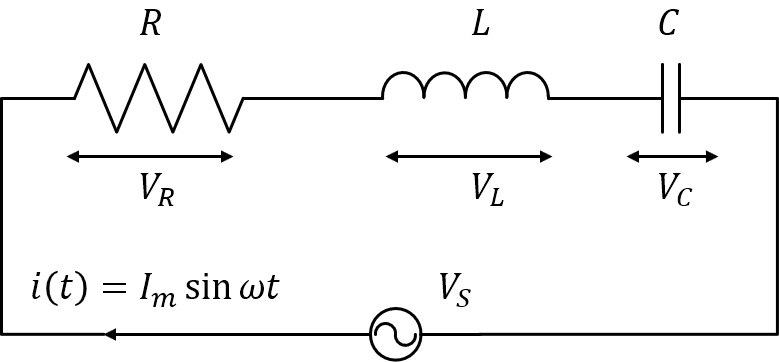
\includegraphics[scale=1]{circuit-1.png}
\end{figure}
The total voltage in RLC circuit is not equal to algebraic sum of voltages across the resistor, the inductor and the capacitor; but it is a vector sum because, in case of resistor the voltage is in phase with the current, for inductor the voltage leads the current by $ 90^\circ $ and for capacitor, the voltage lags behind the current by $ 90^\circ $.

So, voltages in each component are not in phase with each other; so they cannot be added arithmetically. The figure below shows the phasor diagram of series RLC circuit. For drawing the phasor diagram for RLC series circuit, the current is taken as reference because, in series circuit the current in each element remains the same and the corresponding voltage vectors for each component        are        drawn        in        reference        to        common        current         vector.
\[{V_S}^2={V_R}^2+\left( V_L-V_C \right)^2\qquad(\text{if }V_L>V_C)\]
\[{V_S}^2={V_R}^2+\left( V_L-V_C \right)^2\qquad(\text{if }V_L>V_C)\]
Where, $ V_R=IR $, $ V_L=IX_L $, $ V_C=IX_C $
\begin{figure}[ht]
    \centering
    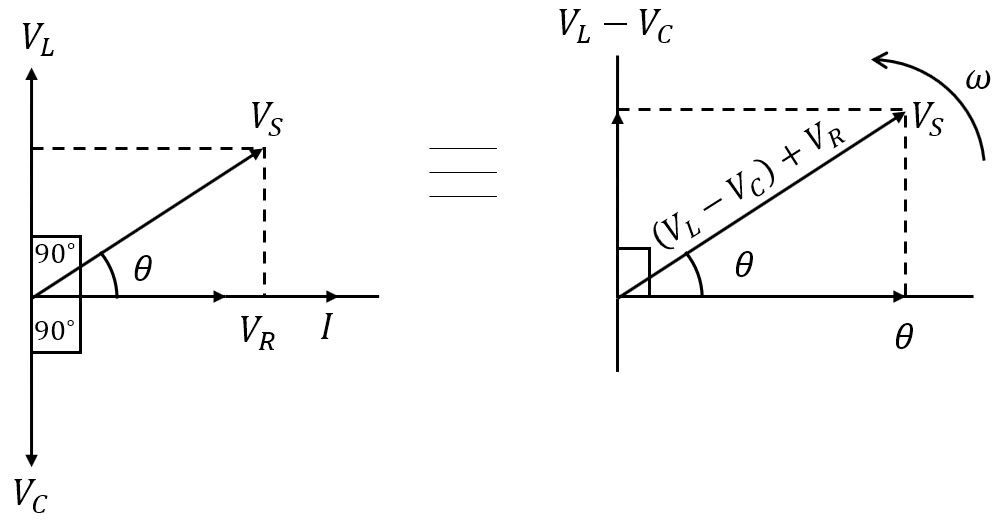
\includegraphics[scale=1]{phasor-1.png}
\end{figure}
The Impedance for a Series RLC Circuit
\begin{figure}[ht]
    \centering
    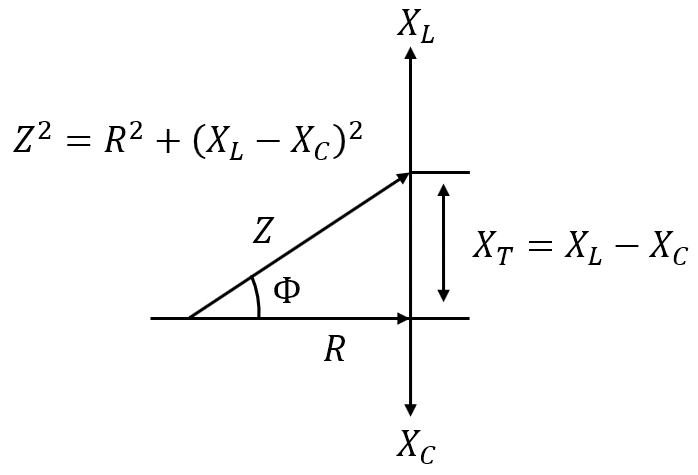
\includegraphics[scale=.75]{phasor-1.1.png}
\end{figure}
The impedance $ Z $ of a series RLC circuit is defined as opposition to the flow of current due circuit resistance $ R $, inductive reactance, $ X_L $ and capacitive reactance, $ X_C $. If the inductive reactance is greater than the capacitive reactance i.e. $ X_L > X_C $, then the RLC circuit has lagging phase angle and if the capacitive reactance is greater than the inductive reactance i.e. $ X_C > X_L $ then, the RLC circuit have leading phase angle and if both inductive and capacitive are same i.e. $ X_L = X_C $ then circuit will behave as purely resistive circuit.

We Know that
\[{V_S}^2={V_R}^2+\left( V_L-V_C \right)^2\]
Where,
\[V_R=IR,\,V_L=IX_L,\,V_C=IX_C\]
Substituting the values
\begin{align*}
    {V_S}^2&=(IR)^2+\left( IX_L-IX_C \right)^2\\
    \Rightarrow\,{V_S}&=I\sqrt{R^2+\left( X_L-X_C \right)^2}\\
    \text{or, impedance }Z&=\sqrt{R^2+\left( X_L-X_C \right)^2}
\end{align*}
\section{Parallel RLC Circuit}
In parallel RLC Circuit the resistor, inductor and capacitor are connected in parallel across a voltage supply. The parallel RLC circuit is exactly opposite to the series RLC circuit. The applied voltage remains the same across all components and the supply current gets divided.

The total current drawn from the supply is not equal to mathematical sum of the current flowing in the individual component, but it is equal to its vector sum of all the currents, as the current flowing in resistor, inductor and capacitor are not in the same phase with each other; so they cannot be added arithmetically.
\begin{figure}[ht]
    \centering
    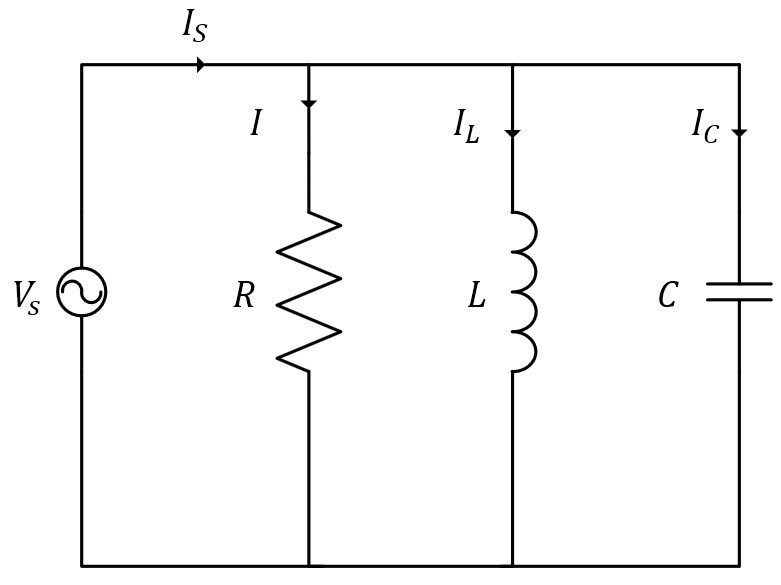
\includegraphics[scale=1]{circuit-2.png}
\end{figure}
Phasor diagram of parallel RLC circuit,\\
$ I_R $ is the current flowing in the resistor, $ R $ in amps.\\
$ I_C $ is the current flowing in the capacitor, $ C $ in amps.\\
$ I_L $ is the current flowing in the inductor, $ L $ in amps.\\
$ I_S $ is the supply current in amps.\\
In the parallel RLC circuit, all the components are connected in parallel; so the voltage across each element is same. Therefore, for drawing phasor diagram, take voltage as reference vector and all the other currents i.e $ I_R $, $ I_C $, $ I_L $ are drawn relative to this voltage vector. The current through each element can be found using Kirchhoff's Current Law, which states that the sum of currents entering a junction or node is equal to the sum of current leaving that node.
\begin{figure}[ht]
    \centering
    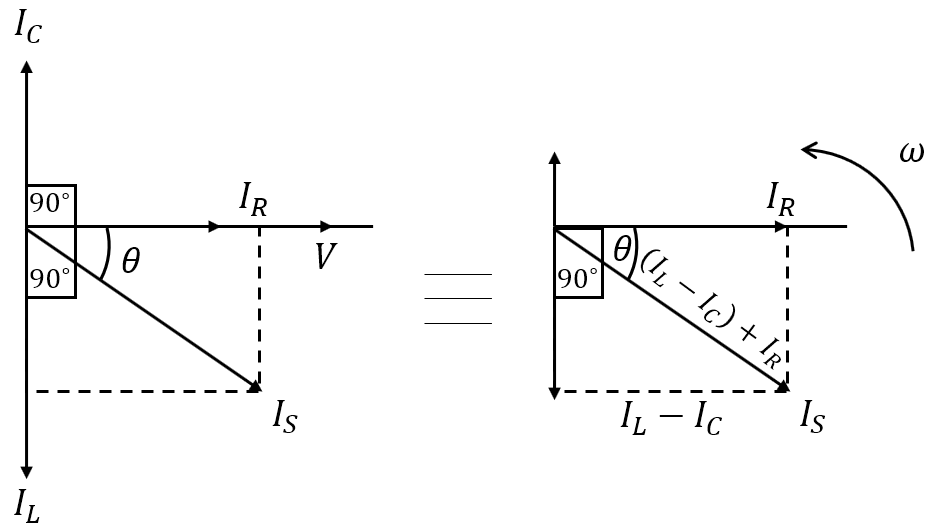
\includegraphics[scale=1]{phasor-2.png}
\end{figure}
\[{I_S}^2={I_R}^2+\left( I_L-I_C \right)^2\]
Now,
\[I_R=\frac{V}{R},\quad I_C=\frac{V}{X_C},\quad I_L=\frac{V}{X_L}\]
\[I_S=\sqrt{\frac{V^2}{R^2}+\left( \frac{V}{X_L}-\frac{V}{X_C} \right)^2}\]
So,
\[\text{admitance, }\frac{1}{Z}=\frac{I_S}{V}=Y=\sqrt{\frac{1}{R^2}+\left( \frac{1}{X_L}-\frac{1}{X_C} \right)^2}\]
As shown above in the equation of impedance, $ Z $ of a parallel RLC circuit; each element has reciprocal of impedance $ (1 / Z) $ i.e. admittance, $ Y $. So in parallel RLC circuit, it is convenient to use admittance instead of impedance.
\end{document}